\documentclass[conference]{IEEEtran}
\IEEEoverridecommandlockouts
\usepackage[utf8]{inputenc}
\usepackage[T1]{fontenc}
\usepackage[spanish,es-tabla,es-nodecimaldot]{babel}
\usepackage{amsmath,amssymb}
\usepackage{graphicx}
\usepackage{booktabs}
\usepackage{multirow}
\usepackage{array}
\usepackage{cite}
\usepackage[hidelinks]{hyperref}
\usepackage{xurl}

\newcommand{\code}[1]{\texttt{#1}}

\markboth{Modelos y Simulación de Sistemas II --- Proyecto de aula --- Entregable II}{}

\begin{document}

\title{PHA Predictor: clasificación de asteroides potencialmente peligrosos con datos de la NASA}

\author{\IEEEauthorblockN{Eliana Maria Brand Agudelo, Jilberth Ferney Alzate Castaño y Juan Esteban Gil Quintero}
\IEEEauthorblockA{Modelos y Simulación de Sistemas II, Departamento de Ingeniería de Sistemas, Universidad de Antioquia, Colombia\\
Repositorio: \url{https://github.com/siderbrand/pha-predictor-nasa-neo}}}

\maketitle

\begin{abstract}
Se aborda la clasificación binaria de asteroides potencialmente peligrosos (PHA) con la base \emph{NASA -- Nearest Earth Objects}, en la que cada uno de los 27\,423 asteroides aparece en promedio 3.3 veces, una por cada aproximación a la Tierra. Se comparan cinco modelos (regresión logística, KNN, Random Forest, red neuronal y SVM) con una partición agrupada por asteroide en entrenamiento, validación y prueba, y se evalúan de dos maneras: por aproximación y por asteroide, agregando las probabilidades de sus filas y ponderando cada asteroide por igual en el ajuste. Todas las decisiones se toman con validación: por asteroide, el Random Forest es el mejor modelo (PR-AUC 0.605), y al ampliar su malla y agregar por el máximo, porque una sola aproximación cercana basta para acotar la distancia mínima de intersección orbital (MOID), su PR-AUC sube a 0.701. Las cinco variables contienen solo tres dimensiones independientes; seleccionarlas conserva el desempeño, mientras que PCA perjudica al Random Forest y UMAP no mejora. Evaluado una única vez en asteroides no vistos, el modelo definido alcanza ROC-AUC 0.952, PR-AUC 0.669 y $F_1$ 0.591, en línea con su validación. La ausencia del MOID en la base fija un techo práctico de desempeño.
\end{abstract}

\begin{IEEEkeywords}
Asteroides potencialmente peligrosos, clasificación binaria, aprendizaje supervisado, datos desbalanceados, datos agrupados, PCA, UMAP.
\end{IEEEkeywords}

% =====================================================================
\section{Descripción del problema}

Un asteroide cercano a la Tierra se considera \emph{potencialmente peligroso} cuando cumple dos condiciones a la vez: su distancia mínima de intersección orbital (MOID) con la Tierra es de 0.05\,ua o menos, unos 7.5 millones de kilómetros, y su magnitud absoluta es $H\le 22$ \cite{cneos}. Cada condición responde a una de las dos preguntas que definen el riesgo de un impacto: si puede ocurrir y cuánto daño causaría.

La primera es geométrica. El MOID es la menor distancia entre las órbitas de la Tierra y del asteroide, sin importar dónde esté cada uno en un momento dado. Un objeto cuyo MOID supera 0.05\,ua no puede, mientras su órbita no cambie, acercarse más que eso; uno por debajo del umbral tiene una órbita que pasa cerca de la terrestre, y como las perturbaciones de los planetas modifican las órbitas con el tiempo, un MOID pequeño hoy es la condición necesaria para un impacto en las próximas décadas o siglos. Por eso el umbral se fija con un margen amplio y no en cero.

La segunda condición es de energía. La magnitud absoluta mide el brillo intrínseco del asteroide y, con un albedo supuesto, su tamaño: $H=22$ corresponde a unos 140\,m de diámetro. La energía de un impacto es la energía cinética del objeto, $E=\tfrac12\,\rho\,\tfrac{\pi}{6}D^{3}v^{2}$, de modo que crece con el cubo del diámetro y el cuadrado de la velocidad. Con la velocidad mediana de esta base (12.3\,km/s) y una densidad rocosa típica de 2\,600\,kg/m$^3$, un asteroide de 140\,m liberaría unos $2.8\times10^{17}$\,J, cerca de 67 megatones de TNT. Como referencia, el objeto de unos 20\,m que estalló sobre Cheliábinsk en 2013 liberó alrededor de 500 kilotones, dañó 7\,200 edificios y envió a 1\,500 personas a centros de salud \cite{chelyabinsk}; un objeto de 140\,m concentra más de cien veces esa energía. A esa escala el daño ya no es local sino regional, comparable a la destrucción de buena parte de un país o a un tsunami si el impacto es en el océano, y por esa razón el Congreso de Estados Unidos ordenó en 2005 a la NASA catalogar el 90\,\% de los objetos cercanos de 140\,m o más \cite{nasem2019,nrc2010}. Ser PHA no significa que el asteroide vaya a chocar: significa que, por su órbita y su tamaño, merece seguimiento prioritario. De hecho, ninguna fila de la base está en el sistema Sentry de la NASA, que lista los objetos con probabilidad de impacto distinta de cero.

Un clasificador automático es útil para \emph{priorizar} ese seguimiento: con pocas variables fáciles de obtener (magnitud, diámetro estimado, velocidad relativa y distancia de paso) ordena qué objetos observar con más detalle y muestra qué variables explican la etiqueta. No reemplaza el cálculo del MOID; como la etiqueta se define con $H$ y MOID y este último no está en la base, el modelo aproxima una regla determinista con variables solo parcialmente informativas, lo que limita el desempeño alcanzable.

La base \emph{NASA -- Nearest Earth Objects} \cite{kaggle} tiene 90\,836 filas y 10 variables (Tabla~\ref{tab:vars}), sin valores faltantes ni filas duplicadas. Cada fila es una aproximación a la Tierra, y las 90\,836 corresponden a solo 27\,423 asteroides, que aparecen entre 1 y 43 veces. Esta estructura condiciona todo el diseño experimental: la etiqueta y $H$ son propiedades del asteroide y no cambian entre sus filas, mientras que la velocidad y la distancia de paso cambian en cada aproximación. Si las filas se repartieran al azar, el mismo asteroide quedaría en entrenamiento y en prueba y el modelo sería evaluado con objetos que ya conoce; con un Random Forest base, esa fuga eleva el ROC-AUC de 0.904 a 0.927. Además, los PHA aparecen en promedio más veces (4.1 filas) que los no PHA (3.2), por lo que las métricas calculadas por fila no pesan igual a todos los asteroides. En la Sección~\ref{sec:metodo} se describe cómo se tratan ambas cosas.

\begin{table}[t]
\centering
\caption{Variables de la base y su tratamiento. Las unidades se validaron contra aproximaciones publicadas por la NASA (Tabla~\ref{tab:unidades}).}
\label{tab:vars}
\footnotesize
\begin{tabular}{@{}p{0.33\columnwidth}p{0.36\columnwidth}p{0.22\columnwidth}@{}}
\toprule
Variable & Significado (tipo, unidad) & Tratamiento\\
\midrule
\code{id} & Identificador del asteroide (entero) & Grupo de la partición\\
\code{name} & Designación (texto) & Excluida\\
\code{est\_diameter\_min} & Diámetro estimado mínimo (continua, km) & $\log_{10}$, z-score\\
\code{est\_diameter\_max} & Diámetro estimado máximo (continua, km) & $\log_{10}$, z-score\\
\code{relative\_velocity} & Velocidad relativa a la Tierra (continua, km/h) & z-score\\
\code{miss\_distance} & Distancia de paso al centro de la Tierra (continua, km) & z-score\\
\code{orbiting\_body} & Cuerpo orbitado, siempre \emph{Earth} & Se elimina\\
\code{sentry\_object} & En el sistema Sentry, siempre falso & Se elimina\\
\code{absolute\_magnitude} & Magnitud absoluta $H$ (continua, mag) & z-score\\
\code{hazardous} & Etiqueta PHA (booleana) & 0/1\\
\bottomrule
\end{tabular}
\end{table}

El análisis exploratorio (notebook \code{entregable1.ipynb}) arroja cuatro hallazgos que orientan el resto del trabajo. Las clases están desbalanceadas: el 9.7\,\% de las filas y el 7.9\,\% de los asteroides son PHA, así que un clasificador que siempre responde ``no peligroso'' acierta el 90.3\,\% de las filas y el 92.1\,\% de los asteroides (Fig.~\ref{fig:eda}a). Los dos diámetros no son mediciones sino una función de $H$: la fórmula $D=1329\,p^{-1/2}\,10^{-H/5}$\,km los reproduce con albedos $p=0.05$ y $p=0.25$ con un error relativo de $5\times10^{-8}$, de modo que solo hay tres variables independientes ($H$, velocidad y distancia de paso). La fracción de PHA es 0.30 cuando $H\le22$ y 0.0015 cuando $H>22$ (Fig.~\ref{fig:eda}b), es decir, $H\le22$ es casi necesaria pero no suficiente, porque falta el MOID. Por último, la capacidad de discriminar de cada variable por separado es desigual: el AUC univariado es 0.865 para $H$, 0.679 para la velocidad y 0.542 para la distancia de paso.

\begin{figure}[t]
\centering
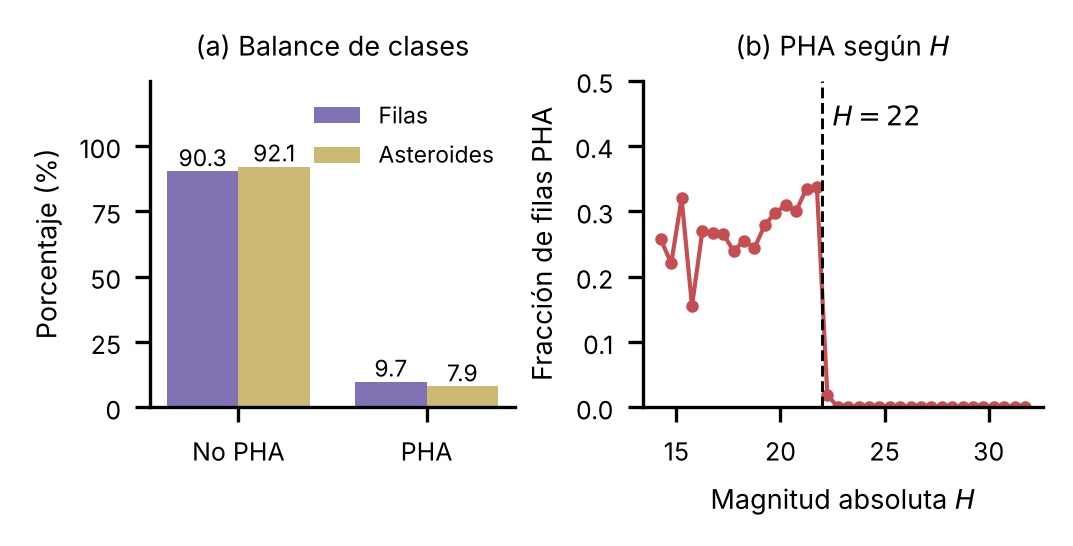
\includegraphics[width=\columnwidth]{figuras/fig1_eda.png}
\caption{(a) Balance de clases por fila y por asteroide. (b) Fracción de filas PHA según la magnitud absoluta $H$ (intervalos de 0.5 mag con al menos 30 filas).}
\label{fig:eda}
\end{figure}

Las unidades merecían una comprobación aparte, porque Kaggle indica kilómetros para los diámetros y la distancia, pero no declara la unidad de la velocidad. Se buscaron en la base tres aproximaciones bien documentadas y se compararon con las cifras publicadas (Tabla~\ref{tab:unidades}). Las distancias coinciden si la columna está en kilómetros medidos desde el centro de la Tierra, y la velocidad coincide si está en km/h: 2001 FO32 aparece con 123\,887 y la NASA reporta unos 124\,000\,km/h \cite{fo32}; 2012 DA14 aparece con 28\,152, que son 7.82\,km/s frente a los 7.8\,km/s publicados \cite{da14}. El rango completo respalda la misma lectura: en km/h la velocidad va de 0.06 a 66\,km/s con mediana de 12\,km/s, mientras que en km/s su máximo sería el 79\,\% de la velocidad de la luz.

\begin{table}[t]
\centering
\caption{Validación de unidades con aproximaciones publicadas. Distancia en km desde el centro de la Tierra; velocidad de la base en km/h.}
\label{tab:unidades}
\footnotesize
\setlength{\tabcolsep}{3pt}
\resizebox{\columnwidth}{!}{%
\begin{tabular}{@{}lrlrl@{}}
\toprule
Asteroide (fecha) & Dist. base & Publicada & Vel. base & Publicada\\
\midrule
2012 DA14 (15/02/2013) & 34\,053 & 27\,700 + 6\,371 \cite{da14} & 28\,152 & 7.8\,km/s \cite{da14}\\
2001 FO32 (21/03/2021) & 2\,016\,392 & $\approx 2\times10^6$ \cite{fo32} & 123\,887 & $\approx$124\,000\,km/h \cite{fo32}\\
433 Eros (31/01/2012) & 26\,729\,521 & 26\,729\,000 \cite{eros} & 21\,403 & ---\\
\bottomrule
\end{tabular}}
\end{table}

El problema se plantea como aprendizaje supervisado, en la modalidad de clasificación binaria: dado $\{(\mathbf{x}_i,y_i)\}_{i=1}^{N}$ con $y_i\in\{0,1\}$, se estima $P(y=1\mid\mathbf{x})$ y se decide con $\hat y=\mathbb{1}[f(\mathbf{x})\ge\tau]$. Todas las filas tienen una etiqueta confiable, la clasificación oficial de la NASA, por lo que no se justifica un enfoque no supervisado ni semisupervisado; la salida es discreta, y los costos son asimétricos, pues no detectar un PHA es más grave que una falsa alarma, así que conviene estimar probabilidades y ajustar el umbral $\tau$.

% =====================================================================
\section{Estado del arte}

Se revisaron cuatro trabajos que clasifican PHA con aprendizaje automático (Tabla~\ref{tab:sota}); los dos primeros usan esta misma base y todos plantean una clasificación binaria supervisada. Los ensambles de árboles, Random Forest y \emph{boosting}, obtienen los mejores resultados en tres de los cuatro. Sus cifras, sin embargo, no son comparables entre sí ni con las nuestras. Malakouti \emph{et al.} \cite{malakouti} reportan AUC pero lo interpretan como exactitud; Wang \cite{wang} reporta exactitud sobre una prueba que, por sus métricas casi simétricas por clase, parece balanceada; y Baimam \cite{baimam} muestra que una exactitud de 0.99 puede convivir con una precisión de 0.24 en la clase PHA, algo esperable cuando un clasificador trivial ya logra el 90\,\% en nuestra base. Ninguno de los trabajos que usan esta base describe una partición agrupada por asteroide: el AUC de 0.94 de \cite{malakouti} es del orden del 0.927 que obtuvimos con partición aleatoria, frente a 0.904 al agrupar, y en \cite{buana} el balanceo se aplica antes de partir los datos. Por último, \cite{malakouti} encuentra que \code{miss\_distance} es la variable más importante pese a ser la menos discriminativa por sí sola, una aparente contradicción que se explica en la Sección~\ref{sec:reduccion}. Estas observaciones motivan el diseño que sigue: partición agrupada, métricas centradas en la clase positiva con intervalos de confianza, evaluación por asteroide y comparación frente a un clasificador trivial y a un modelo que solo usa $H$.

\begin{table*}[t]
\centering
\caption{Trabajos previos sobre la clasificación de PHA.}
\label{tab:sota}
\footnotesize
\resizebox{\textwidth}{!}{%
\begin{tabular}{@{}p{0.03\textwidth}p{0.15\textwidth}p{0.2\textwidth}p{0.17\textwidth}p{0.12\textwidth}p{0.23\textwidth}@{}}
\toprule
Ref. & Datos & Técnicas & Validación & Métricas & Resultados\\
\midrule
\cite{malakouti} & Kaggle; enlaza otra base (\emph{NASA asteroids classification}) pero describe 90\,836 filas y 10 columnas, como la nuestra & Extra Trees, Random Forest (RF), LightGBM, Gradient Boosting (GB), AdaBoost; GridSearchCV; atípicos eliminados y Min-Max & 80\,\% con CV de 10 pliegues; 20\,\% restante en validación y prueba (10/10\,\%). Sin partición agrupada & AUC por clase, micro y macro & RF: AUC 0.94 por clase, micro 0.98, macro 0.94; Extra Trees 0.93; LightGBM y GB 0.92; AdaBoost 0.91. El texto llama exactitud al AUC\\
\cite{wang} & Misma base (90\,836$\times$10); sin \code{orbiting\_body} ni \code{sentry\_object} & Regresión logística (LR), KNN, RF, árbol de decisión (DT), Naive Bayes (NB), GB, Voting (RF+DT+GB) & No describe la partición; sus métricas sugieren una prueba balanceada (inferencia nuestra) & Exactitud, precisión, recall, $F_1$ & Exactitud: RF 0.95, Voting 0.94, DT 0.93, GB 0.89 (recall PHA 0.99), KNN 0.79, LR 0.58, NB 0.56\\
\cite{buana} & Kaggle Asteroid Dataset (958\,524 filas) y NeoWs (362\,717; $\approx$13\,\% positivos) & LR, KNN, SVC, RF, CatBoost; MLP, DNN, Conv2D, RNN, LSTM; \emph{bootstrapping} y SMOTE & 80:20; balanceo y escalado descritos antes de la partición & Exactitud, precisión, recall, $F_1$, ROC-AUC & RF y CatBoost: $F_1$ = AUC = 0.99 en ambas bases; DNN $\approx$0.99 de exactitud (NeoWs)\\
\cite{baimam} & JPL Small-Body Database vía Kaggle (958\,524 asteroides; 0.22\,\% PHA; $>$85\,\% de faltantes en diámetro y albedo) & Red neuronal de grafos (kNN, $k=5$); SMOTE y Focal Loss; frente a MLP, GAT e Isolation Forest & 80:20 estratificada; SMOTE solo en entrenamiento & Precisión, recall, $F_1$, AUC & Exactitud 0.99, AUC 0.99; clase PHA: precisión 0.24, recall 0.78, $F_1$ 0.37\\
\bottomrule
\end{tabular}}
\end{table*}

% =====================================================================
\section{Metodología}
\label{sec:metodo}

Las entradas son las cinco variables numéricas, con los diámetros en $\log_{10}$, y todo escalado se ajusta solo con los datos de entrenamiento de cada partición, dentro del modelo. La partición sigue la secuencia entrenamiento, validación y prueba, y en las tres el asteroide completo es la unidad que se reparte (Fig.~\ref{fig:particion}). Primero se reserva el 20\,\% de los asteroides (5\,485 asteroides y 18\,168 filas) como conjunto de prueba. Con el 80\,\% restante, el conjunto de desarrollo, se forman cinco pliegues estratificados por clase y agrupados por \code{id} (\code{StratifiedGroupKFold} de scikit-learn \cite{sklearn}); en cada uno, cuatro partes sirven de entrenamiento para ajustar los parámetros del modelo y la quinta de validación. Un \code{assert} verifica en cada partición que ningún asteroide aparece a la vez en entrenamiento y validación, ni en desarrollo y prueba.

La validación es la única base para decidir. Con ella se comparan los modelos, se eligen los hiperparámetros (mayor PR-AUC media en los cinco pliegues), la forma de agregar las predicciones de un asteroide, la representación de entrada y el umbral, que maximiza $F_1$ sobre las predicciones fuera de muestra. Solo cuando todas esas decisiones están tomadas el modelo queda \emph{definido}: se reentrena con todo el conjunto de desarrollo y se evalúa una única vez en la prueba (Sección~\ref{sec:prueba}). Por eso las tablas de las Secciones~\ref{sec:resultados} y~\ref{sec:reduccion} solo contienen cifras de entrenamiento y validación.

\begin{figure*}[t]
\centering
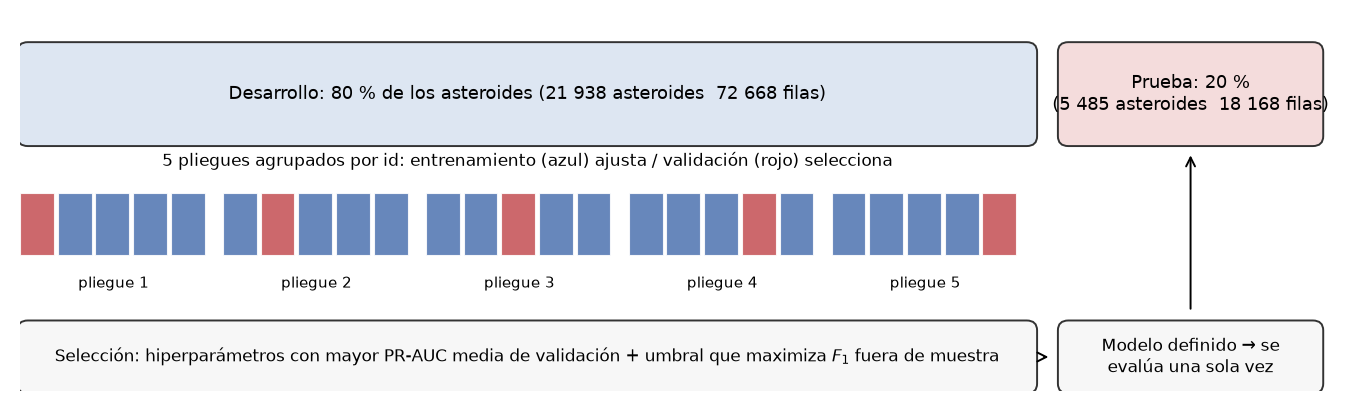
\includegraphics[width=0.85\textwidth]{figuras/fig_particion.png}
\caption{Partición agrupada por asteroide. El entrenamiento ajusta los parámetros, la validación selecciona hiperparámetros y umbral, y la prueba evalúa una sola vez el modelo ya definido.}
\label{fig:particion}
\end{figure*}

Se compara un modelo por familia, con las mallas de la Tabla~\ref{tab:grids}: regresión logística (paramétrico), KNN (no paramétrico), Random Forest (ensamble de árboles), perceptrón multicapa (red neuronal) y SVM con núcleo RBF. El desbalance se trata con pesos de clase en la regresión logística y el SVM y con el ajuste del umbral en todos; no se remuestrea. Solo el SVM se entrena con una submuestra aleatoria de hasta 25\,000 filas, porque su costo crece aproximadamente con el cuadrado del número de ejemplos.

\begin{table*}[t]
\centering
\caption{Modelos, mallas de hiperparámetros y configuración seleccionada por PR-AUC de validación, por fila y por asteroide (con pesos $1/n$). La última fila es la malla ampliada del modelo definido (Sección~\ref{sec:rf}).}
\label{tab:grids}
\footnotesize
\resizebox{\textwidth}{!}{%
\begin{tabular}{@{}llccc@{}}
\toprule
Modelo & Hiperparámetros y valores de la malla & Config. & Seleccionada por fila & Seleccionada por asteroide\\
\midrule
Regresión logística & $C\in\{0.01,0.1,1,10,100\}$; pesos de clase $\in\{$ninguno, balanceado$\}$ & 10 & $C=100$, sin pesos & $C=100$, sin pesos\\
KNN & $k\in\{5,11,25,51,101,201\}$; ponderación $\in\{$uniforme, distancia$\}$ & 12 & $k=201$, distancia & $k=101$, distancia\\
Random Forest (150 árboles) & profundidad máx. $\in\{4,8,12,\infty\}$; hoja mínima $\in\{1,10,50\}$ & 12 & profundidad 8, hoja 1 & profundidad 4, hoja 1\\
Red neuronal (ReLU, Adam, parada temprana) & capas ocultas $\in\{(16),(64),(64,32)\}$; $\alpha\in\{10^{-4},10^{-2},1\}$ & 9 & $(64,32)$, $\alpha=10^{-4}$ & $(64,32)$, $\alpha=10^{-4}$\\
SVM con núcleo RBF & $C\in\{1,10\}$; $\gamma\in\{0.05,0.2,1\}$; pesos de clase $\in\{$ninguno, balanceado$\}$ & 12 & $C=10$, $\gamma=0.2$, sin pesos & $C=10$, $\gamma=0.2$, sin pesos\\
\midrule
Random Forest, malla ampliada & profundidad $\in\{2,3,4,5,6,8,12\}$; hoja $\in\{1,10,50,200\}$; variables por división $\in\{1,2,3,5\}$; agregación $\in\{$media, mediana, máximo$\}$ & 336 & --- & profundidad 5, hoja 50, 3 variables, máximo\\
\bottomrule
\end{tabular}}
\end{table*}

La repetición de asteroides se trata de dos maneras complementarias. La primera evalúa por aproximación, como si cada fila fuera independiente una vez garantizado que ningún asteroide cruza la partición; responde a la pregunta de qué tan bien se clasifica una aproximación nueva. La segunda toma al asteroide como unidad de análisis, que es lo que define la etiqueta. En el ajuste, cada fila recibe un peso $w_i=1/n_{\mathrm{id}(i)}$, normalizado a media 1, de modo que todos los asteroides aportan lo mismo a la función de pérdida, tengan una aproximación o cuarenta. Los pesos se pasan como \code{sample\_weight} a la regresión logística, el Random Forest, la red neuronal y el SVM; como el KNN de scikit-learn no los admite, se implementó una versión en la que el voto de cada vecino se multiplica por su peso. En la predicción, la probabilidad de un asteroide se obtiene agregando las de sus filas, y con ese valor se calculan todas las métricas. La agregación por defecto es el promedio; para el modelo definido se comparan además la mediana y el máximo, que tiene una justificación física: la distancia de paso de cada aproximación es una cota superior del MOID, así que basta una sola aproximación cercana para que el asteroide cumpla la condición orbital de PHA.

La métrica principal es la PR-AUC (precisión promedio), cuyo valor al azar es la prevalencia y que no se infla con los muchos negativos fáciles; el ROC-AUC se reporta como complemento comparable con la literatura. Al umbral elegido se reportan además el $F_1$ de la clase PHA, la precisión, el recall y la exactitud. La exactitud debe leerse frente al 90.3\,\% (por fila) o al 92.1\,\% (por asteroide) del clasificador trivial: con un umbral que busca detectar la mayoría de los PHA, un modelo útil puede tener menos exactitud que ese clasificador. Los intervalos de validación son $\bar x\pm t_{0.975,4}\,s/\sqrt5$ sobre los cinco pliegues, y los de prueba son intervalos percentil al 95\,\% de un \emph{bootstrap} con 500 réplicas en el que se remuestrean asteroides. Como referencias se incluyen un clasificador constante y una regresión logística que usa solo $H$. El notebook \code{entregable2.ipynb} reproduce todas las cifras, tablas y figuras de las Secciones~\ref{sec:metodo} a~\ref{sec:conclusiones}.

% =====================================================================
\section{Resultados}
\label{sec:resultados}

\subsection{Evaluación por aproximación}

La Fig.~\ref{fig:hyper} muestra cómo cambia la PR-AUC de validación con los hiperparámetros cuando cada fila cuenta por separado. En la regresión logística $C$ casi no influye y los pesos de clase no ayudan (0.302 sin pesos frente a 0.291 con ellos). En KNN la PR-AUC crece con $k$ hasta saturar entre 50 y 200 vecinos, y ponderar por distancia supera al voto uniforme. El Random Forest rinde mejor con una profundidad moderada, porque sin límite y con hojas de una fila sobreajusta (0.471). En la red neuronal la mayor capacidad ayuda y una regularización fuerte ($\alpha=1$) perjudica, y en el SVM lo mejor es un $\gamma$ intermedio sin pesos de clase.

\begin{figure*}[t]
\centering
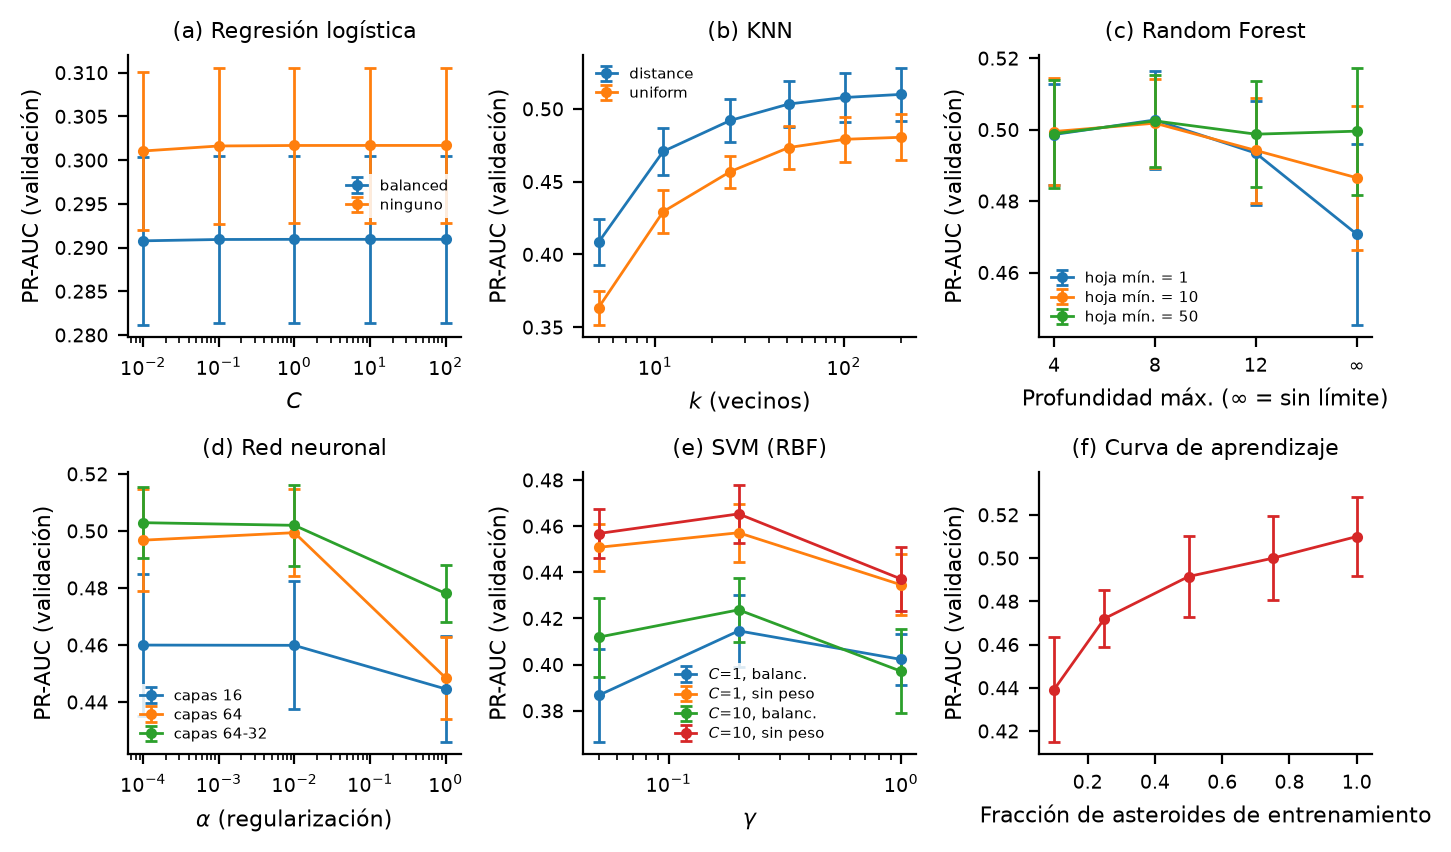
\includegraphics[width=0.85\textwidth]{figuras/fig2_hiperparametros.png}
\caption{Efecto de los hiperparámetros sobre la PR-AUC de validación por fila (media $\pm$ desviación entre los 5 pliegues) y curva de aprendizaje del mejor modelo por fila (KNN).}
\label{fig:hyper}
\end{figure*}

Con la mejor configuración de cada familia (Tabla~\ref{tab:fila} y Fig.~\ref{fig:curvas}), KNN, el Random Forest y la red neuronal empatan dentro de sus intervalos, con PR-AUC de validación de 0.503 a 0.510, ROC-AUC de 0.910 a 0.911 y $F_1\approx0.48$; la regresión logística y el SVM quedan por debajo. Frente al modelo que solo usa $H$ (PR-AUC 0.275) la mejora es clara en PR-AUC, pero pequeña en $F_1$ (0.461 frente a 0.48). Al umbral elegido, los tres mejores modelos detectan entre el 77 y el 91\,\% de los PHA con una precisión de 0.33 a 0.35, de modo que una de cada tres alarmas es real, y su exactitud (0.81 a 0.84) queda por debajo del 0.90 del clasificador trivial, que no detecta ningún PHA. KNN llega a 1.000 en entrenamiento porque, al ponderar por distancia, cada fila es su propio vecino; la red neuronal casi no sobreajusta (0.514 en entrenamiento y 0.503 en validación) y el Random Forest algo más (0.591 y 0.503).

\begin{table*}[t]
\centering
\caption{Evaluación por aproximación (fila). Entrenamiento: media de los pliegues; validación: media $\pm$ IC 95\,\% sobre 5 pliegues. Exactitud del clasificador trivial (todo no PHA): 0.903. La prueba no se usa en esta comparación.}
\label{tab:fila}
\footnotesize
\setlength{\tabcolsep}{3.5pt}
\resizebox{\textwidth}{!}{%
\begin{tabular}{@{}lcccccccccc@{}}
\toprule
& \multicolumn{2}{c}{PR-AUC} & \multicolumn{2}{c}{ROC-AUC} & \multicolumn{2}{c}{$F_1$ (clase PHA)} & Precisión & Recall & Exactitud & Umbral\\
\cmidrule(lr){2-3}\cmidrule(lr){4-5}\cmidrule(lr){6-7}\cmidrule(lr){8-10}
Modelo & Entren. & Validación & Entren. & Validación & Entren. & Validación & \multicolumn{3}{c}{Validación} & \\
\midrule
Regresión logística & 0.300 & 0.302$\pm$0.011 & 0.873 & 0.873$\pm$0.005 & 0.448 & 0.448$\pm$0.008 & 0.309$\pm$0.009 & 0.818$\pm$0.024 & 0.804 & 0.121\\
KNN & 1.000 & 0.510$\pm$0.023 & 1.000 & 0.911$\pm$0.007 & 1.000 & 0.481$\pm$0.014 & 0.328$\pm$0.013 & 0.903$\pm$0.010 & 0.810 & 0.199\\
Random Forest & 0.591 & 0.503$\pm$0.017 & 0.932 & 0.910$\pm$0.008 & 0.521 & 0.485$\pm$0.015 & 0.354$\pm$0.013 & 0.767$\pm$0.018 & 0.841 & 0.267\\
Red neuronal & 0.514 & 0.503$\pm$0.015 & 0.914 & 0.910$\pm$0.006 & 0.484 & 0.481$\pm$0.016 & 0.327$\pm$0.018 & 0.910$\pm$0.039 & 0.808 & 0.199\\
SVM (RBF) & 0.472 & 0.465$\pm$0.016 & 0.890 & 0.888$\pm$0.005 & 0.445 & 0.442$\pm$0.008 & 0.341$\pm$0.012 & 0.630$\pm$0.021 & 0.845 & $-1.002$\\
Solo $H$ (reg. log.) & 0.272 & 0.275$\pm$0.010 & 0.863 & 0.863$\pm$0.006 & 0.460 & 0.461$\pm$0.015 & 0.301$\pm$0.013 & 0.984$\pm$0.016 & 0.776 & 0.098\\
Constante (todo PHA) & 0.097 & 0.097$\pm$0.000 & 0.500 & 0.500$\pm$0.000 & 0.177 & 0.177$\pm$0.000 & 0.097$\pm$0.000 & 1.000$\pm$0.000 & 0.097 & ---\\
\bottomrule
\end{tabular}}
\end{table*}

\begin{figure*}[t]
\centering
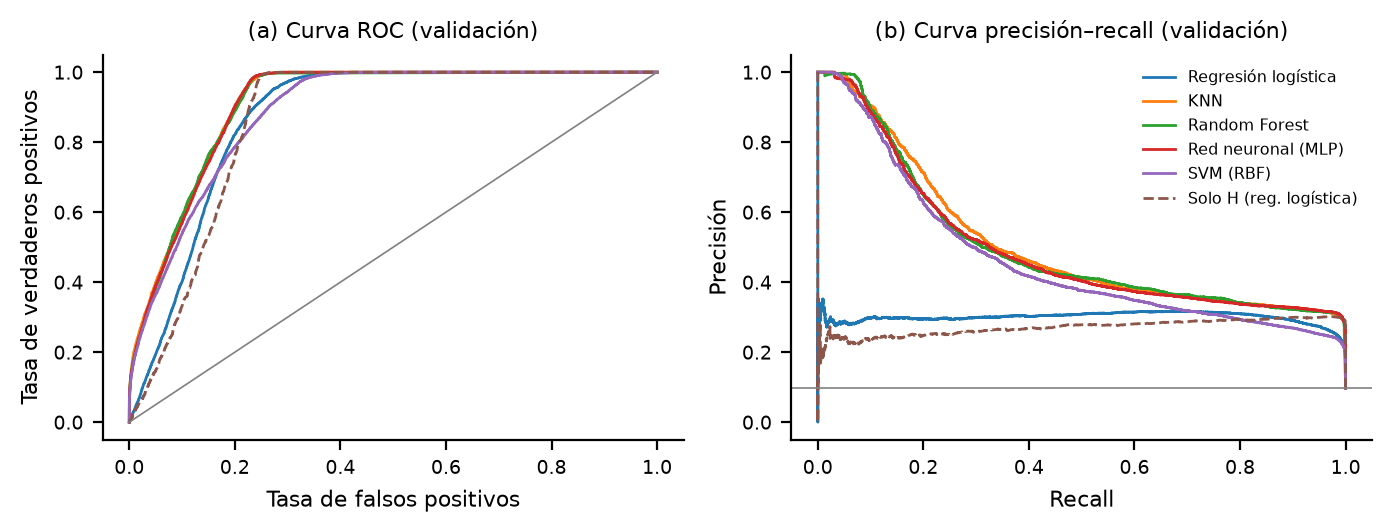
\includegraphics[width=0.85\textwidth]{figuras/fig3_curvas.png}
\caption{Curvas ROC y precisión--recall por fila con las predicciones fuera de muestra del conjunto de desarrollo (validación). La línea gris marca el desempeño al azar.}
\label{fig:curvas}
\end{figure*}

\subsection{Evaluación por asteroide}

Tomar al asteroide como unidad cambia el panorama (Tabla~\ref{tab:asteroide} y Fig.~\ref{fig:asteroide}). Al promediar las probabilidades de todas las aproximaciones de un objeto, los cuatro modelos no lineales suben a una PR-AUC de validación de 0.55 a 0.61 y a un ROC-AUC de 0.94, frente a 0.47--0.51 y 0.89--0.91 por fila. Las dos cifras miden poblaciones distintas, pero la mejora es coherente con el problema: el promedio suaviza las predicciones ruidosas de aproximaciones aisladas de un objeto cuya etiqueta no cambia. Los pesos $1/n$ aportan menos. Con hiperparámetros elegidos por asteroide, la PR-AUC de validación mejora en los cinco modelos, pero solo entre 0.005 y 0.016 (de 0.589 a 0.605 en el Random Forest), dentro de los intervalos, y el $F_1$ incluso baja ligeramente en tres de ellos. Los pesos sí cambiaron la configuración elegida en dos modelos: KNN pasó de 201 a 101 vecinos y el Random Forest de profundidad 8 a 4 (Tabla~\ref{tab:grids}), lo que indica que, al dejar de sobrerrepresentar a los asteroides con muchas aproximaciones, conviene un modelo algo más simple.

Ningún modelo gana en todas las métricas. Ordenados por su valor de validación con pesos, el Random Forest es el mejor en PR-AUC (0.605), la red neuronal en ROC-AUC (0.943) y el SVM en $F_1$ (0.595), precisión (0.571) y exactitud (0.933); la regresión logística tiene el mayor recall (0.83), pero solo porque marca muchos asteroides, con una precisión de 0.27. El criterio, sin embargo, se fijó antes de ver los resultados: la PR-AUC, que no depende del umbral y no se infla con el desbalance. Por ese criterio el modelo elegido es el Random Forest, seguido del SVM (0.591), y sobre él se toman las decisiones restantes.

\begin{table*}[t]
\centering
\caption{Evaluación por asteroide en validación (media $\pm$ IC 95\,\% sobre 5 pliegues; probabilidad promedio de sus filas). ``Sin pesos'': modelos de la Tabla~\ref{tab:fila}. ``Con pesos'': pesos $1/n$ e hiperparámetros elegidos por asteroide. Exactitud del clasificador trivial: 0.921. En negrita, el mejor valor de cada métrica con pesos (sin contar el recall, que la regresión logística gana a costa de su precisión).}
\label{tab:asteroide}
\footnotesize
\setlength{\tabcolsep}{3pt}
\resizebox{\textwidth}{!}{%
\begin{tabular}{@{}llcccccc@{}}
\toprule
Estrategia & Modelo & PR-AUC & ROC-AUC & $F_1$ & Precisión & Recall & Exactitud\\
\midrule
Sin pesos & Regresión logística & 0.259$\pm$0.011 & 0.876$\pm$0.005 & 0.403$\pm$0.010 & 0.262$\pm$0.010 & 0.876$\pm$0.014 & 0.794$\pm$0.011\\
 & KNN & 0.550$\pm$0.027 & 0.937$\pm$0.003 & 0.531$\pm$0.009 & 0.459$\pm$0.024 & 0.631$\pm$0.037 & 0.912$\pm$0.006\\
 & Random Forest & 0.589$\pm$0.020 & 0.938$\pm$0.002 & 0.558$\pm$0.014 & 0.533$\pm$0.036 & 0.587$\pm$0.023 & 0.926$\pm$0.006\\
 & Red neuronal & 0.569$\pm$0.022 & 0.941$\pm$0.004 & 0.557$\pm$0.036 & 0.530$\pm$0.112 & 0.606$\pm$0.084 & 0.923$\pm$0.020\\
 & SVM (RBF) & 0.586$\pm$0.035 & 0.937$\pm$0.005 & 0.591$\pm$0.020 & 0.561$\pm$0.052 & 0.626$\pm$0.030 & 0.931$\pm$0.009\\
\midrule
Con pesos $1/n$ & Regresión logística & 0.275$\pm$0.013 & 0.883$\pm$0.005 & 0.412$\pm$0.011 & 0.274$\pm$0.011 & 0.831$\pm$0.024 & 0.812$\pm$0.011\\
 & KNN & 0.561$\pm$0.025 & 0.941$\pm$0.004 & 0.529$\pm$0.011 & 0.422$\pm$0.022 & 0.711$\pm$0.033 & 0.900$\pm$0.008\\
 & Random Forest & \textbf{0.605}$\pm$0.016 & 0.941$\pm$0.004 & 0.556$\pm$0.031 & 0.555$\pm$0.071 & 0.561$\pm$0.019 & 0.929$\pm$0.012\\
 & Red neuronal & 0.577$\pm$0.036 & \textbf{0.943}$\pm$0.004 & 0.527$\pm$0.012 & 0.524$\pm$0.135 & 0.569$\pm$0.146 & 0.919$\pm$0.024\\
 & SVM (RBF) & 0.591$\pm$0.031 & 0.938$\pm$0.004 & \textbf{0.595}$\pm$0.024 & \textbf{0.571}$\pm$0.040 & 0.622$\pm$0.031 & \textbf{0.933}$\pm$0.006\\
 & Solo $H$ (reg. log.) & 0.216$\pm$0.008 & 0.849$\pm$0.006 & 0.385$\pm$0.012 & 0.239$\pm$0.009 & 0.987$\pm$0.016 & 0.750$\pm$0.014\\
\bottomrule
\end{tabular}}
\end{table*}

\begin{figure*}[t]
\centering
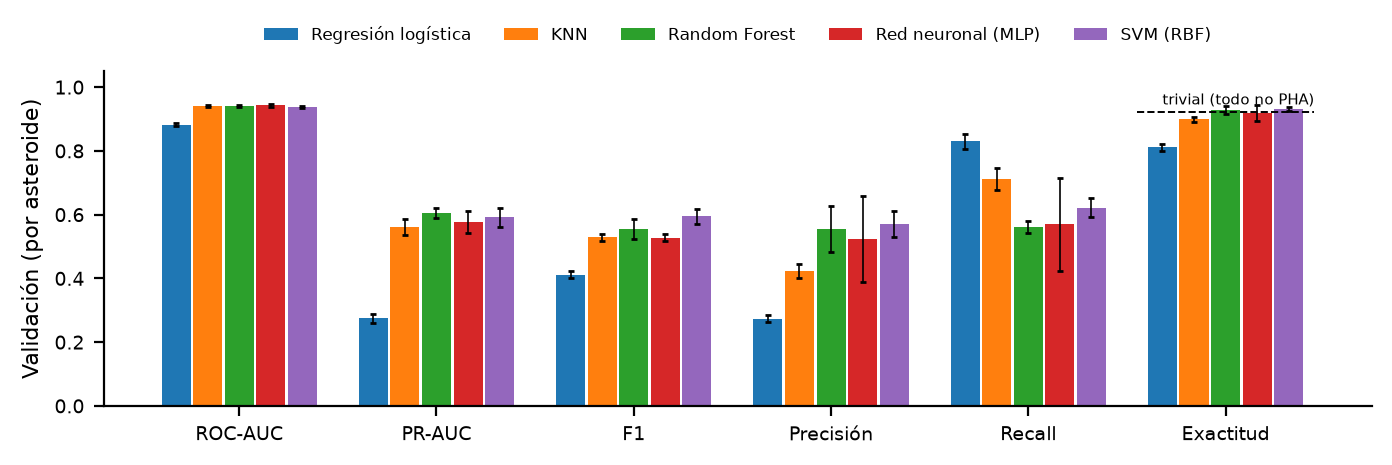
\includegraphics[width=0.85\textwidth]{figuras/fig_asteroide.png}
\caption{Métricas de validación por asteroide con pesos $1/n$ (media $\pm$ IC 95\,\% sobre 5 pliegues). La línea discontinua en la exactitud es el clasificador trivial.}
\label{fig:asteroide}
\end{figure*}

\subsection{Modelo definido: Random Forest}
\label{sec:rf}

Antes de dar el Random Forest por definido había que resolver un problema de la búsqueda: su mejor configuración por asteroide quedó en el borde de la malla, con la profundidad mínima probada (4), lo que deja abierta la posibilidad de que un árbol aún más simple, o uno algo más profundo con otras restricciones, rinda mejor. Por eso la malla se amplió alrededor de ese punto (última fila de la Tabla~\ref{tab:grids}) con dos hiperparámetros que la original no exploraba, el número de variables candidatas en cada división y la forma de agregar las probabilidades de un asteroide, para un total de 336 combinaciones evaluadas con los mismos pliegues y pesos.

La configuración ganadora quedó en el interior de la malla, con profundidad 5, hoja mínima de 50 filas y 3 variables por división, y la Fig.~\ref{fig:rf} muestra que alrededor de ella la superficie es plana: entre profundidades 4 y 8 las diferencias son menores que la variación entre pliegues, mientras que con profundidad 2 o 3 el modelo se queda corto. El cambio decisivo no vino de los árboles sino de la agregación. Con la misma configuración, tomar el \emph{máximo} de las probabilidades de un asteroide da una PR-AUC de validación de 0.701, frente a 0.613 con la media y 0.515 con la mediana. La explicación es la misma que justifica la definición de PHA: una sola aproximación que pase cerca basta para acotar el MOID, y promediarla con las demás diluye justamente la evidencia más informativa. Dos comprobaciones cierran la búsqueda. Con 500 árboles la PR-AUC es idéntica (0.7007 frente a 0.7008 con 150), así que se mantienen 150, y la curva de aprendizaje (Fig.~\ref{fig:rf}c) sube rápido hasta la mitad de los datos y luego se estanca: de 75 a 100\,\% gana 0.004, menos que su desviación entre pliegues (0.008).

Frente al Random Forest de la Sección anterior, el modelo definido mejora todas las métricas de validación por asteroide: la PR-AUC pasa de 0.605 a 0.701, el ROC-AUC de 0.941 a 0.953, el $F_1$ de 0.556 a 0.602 y el recall de 0.561 a 0.609, con una exactitud de 0.936. La diferencia entre entrenamiento y validación es pequeña (PR-AUC 0.713 y 0.701), de modo que el modelo no sobreajusta.

\begin{figure*}[t]
\centering
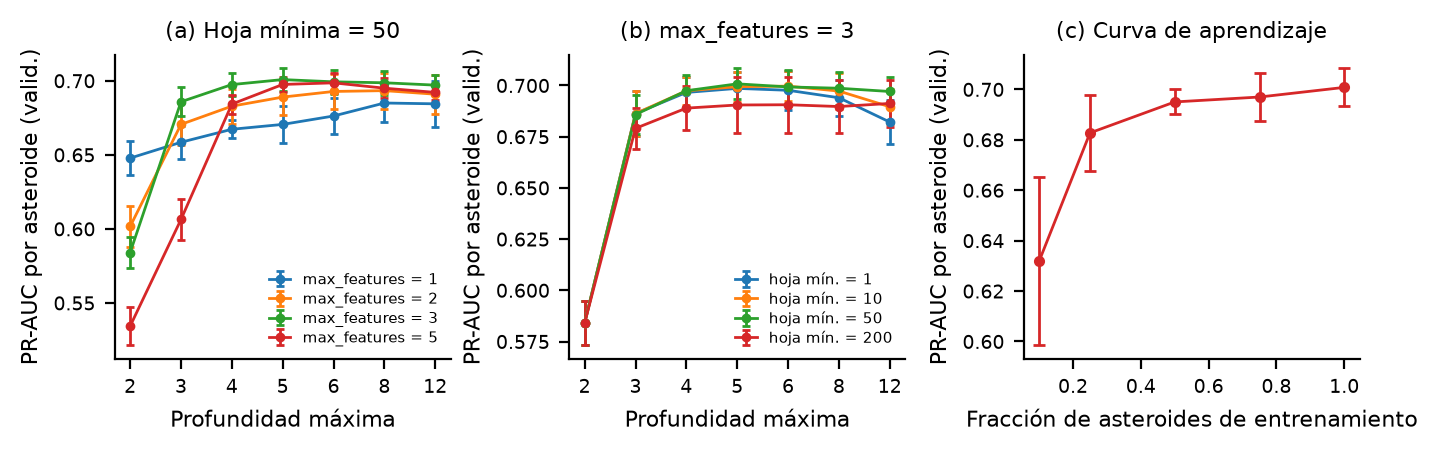
\includegraphics[width=0.85\textwidth]{figuras/fig_rf.png}
\caption{Malla ampliada del Random Forest con agregación por máximo (PR-AUC por asteroide en validación, media $\pm$ desviación entre pliegues). (a) Profundidad y variables por división con hoja mínima 50. (b) Profundidad y hoja mínima con 3 variables por división. (c) Curva de aprendizaje del modelo definido.}
\label{fig:rf}
\end{figure*}

Como la etiqueta depende del MOID, ausente en la base, no puede calcularse un máximo teórico, pero varias evidencias apuntan a un techo práctico. Familias de modelos muy distintas convergen al mismo valor, tanto por fila como por asteroide; las curvas de aprendizaje se estancan, la del mejor modelo por fila (Fig.~\ref{fig:hyper}f) y la del modelo definido; y dentro del grupo $H\le22$, el único donde la clase es realmente incierta (32\,\% de las filas de desarrollo, 30\,\% de ellas PHA), el mejor modelo por fila alcanza en validación un ROC-AUC de 0.65, mientras que $H$ sola no tiene señal (0.46).

% =====================================================================
\section{Reducción de dimensión}
\label{sec:reduccion}

La reducción de dimensión se evaluó con los dos mejores modelos por asteroide, el Random Forest definido y el SVM, con sus hiperparámetros ya fijados, pesos $1/n$ y métricas por asteroide en validación. El análisis individual de las variables (Tabla~\ref{tab:indiv}) confirma que $H$ y los dos diámetros son las más discriminativas, con AUC univariado de 0.863, y que son equivalentes entre sí ($|\rho|=1$): eliminar cualquiera deja la PR-AUC igual, de modo que dos de las tres sobran. La velocidad discrimina de forma moderada (AUC 0.683) y la distancia de paso es la más débil (AUC 0.542, información mutua 0.006), lo que la haría candidata a eliminarse; sin embargo, quitarla del Random Forest reduce la PR-AUC por asteroide en 0.334, más que cualquier otra variable. La razón es física: la distancia de paso en una aproximación nunca es menor que el MOID del asteroide, así que si un objeto con $H\le22$ pasa a menos de 0.05\,ua es necesariamente PHA. En el desarrollo, el 97.8\,\% de las 494 filas que cumplen ambas condiciones son PHA, aunque solo cubren el 6.8\,\% de las filas PHA; contado por asteroide, usando la menor distancia de sus aproximaciones, la misma regla identifica el 24.4\,\% de los asteroides PHA con una precisión de 0.977. Es una interacción que ninguna medida univariada captura, que explica la importancia que \cite{malakouti} atribuye a esta variable y que respalda la agregación por máximo. Por eso solo se descartan las variables redundantes, y la selección resultante, $H$, velocidad y distancia de paso, rinde lo mismo que las cinco variables (PR-AUC 0.698 frente a 0.701).

\begin{table}[t]
\centering
\caption{Análisis individual de variables (desarrollo): correlación de Spearman con la etiqueta, AUC univariado, información mutua (IM), máxima correlación con otra variable y cambio de PR-AUC por asteroide de validación al eliminarla del Random Forest definido.}
\label{tab:indiv}
\footnotesize
\begin{tabular}{@{}lccccc@{}}
\toprule
Variable & $|\rho|$ & AUC & IM & Máx. $|\rho|$ & $\Delta$ PR-AUC\\
\midrule
$\log_{10} d_{\min}$ & 0.373 & 0.863 & 0.147 & 1.000 & 0.000\\
$\log_{10} d_{\max}$ & 0.373 & 0.863 & 0.146 & 1.000 & 0.000\\
velocidad & 0.188 & 0.683 & 0.022 & 0.339 & $-0.013$\\
dist. de paso & 0.043 & 0.542 & 0.006 & 0.327 & $-0.334$\\
$H$ & 0.373 & 0.863 & 0.145 & 1.000 & 0.000\\
\bottomrule
\end{tabular}
\end{table}

Para la extracción lineal se aplicó PCA a las cinco variables estandarizadas, ajustado dentro de cada pliegue. El número de componentes se eligió como el menor $k$ con varianza explicada acumulada de al menos 99\,\% en desarrollo, contrastado con el desempeño de validación (Fig.~\ref{fig:pca}). Los componentes explican 66.0, 20.8, 13.2, 0 y 0\,\% de la varianza, de modo que la dimensión efectiva es 3 y $k=3$ cumple el criterio. En el SVM, tres componentes casi conservan el desempeño (PR-AUC 0.575 frente a 0.591, dentro del intervalo), pero en el Random Forest la PR-AUC cae de 0.701 a 0.589 (Tabla~\ref{tab:reduccion}), y con dos componentes ambos modelos se desploman. La diferencia entre los dos modelos tiene una explicación concreta: PCA rota los ejes y mezcla $H$ con la distancia de paso, mientras que los árboles aprovechan cortes paralelos a los ejes, como $H\le22$ y distancia $\le0.05$\,ua; al perderlos, el Random Forest necesita muchos más cortes para aproximar la misma frontera. PCA recupera, por tanto, la misma dimensión que la selección manual, pero en una base que no le conviene al modelo definido.

\begin{figure}[t]
\centering
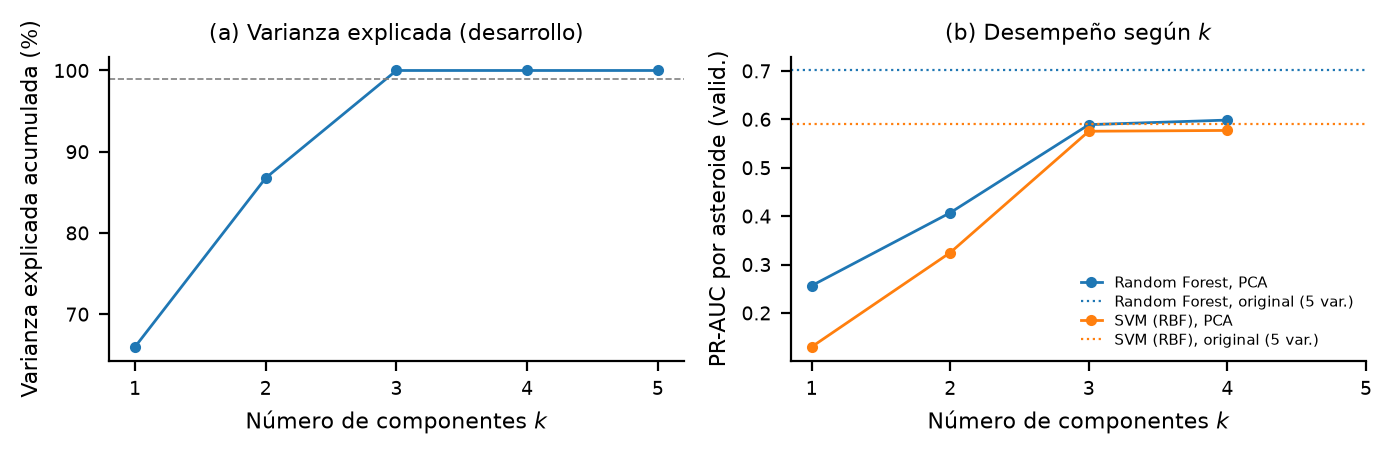
\includegraphics[width=\columnwidth]{figuras/fig4_pca.png}
\caption{PCA. (a) Varianza explicada acumulada en desarrollo. (b) PR-AUC por asteroide de validación según el número de componentes $k$ para el Random Forest definido y el SVM; las líneas punteadas son los modelos con las variables originales.}
\label{fig:pca}
\end{figure}

Para la extracción no lineal se usó UMAP \cite{umap} (\code{n\_neighbors=15}, \code{min\_dist=0.1}, sin usar la etiqueta), ajustado dentro de cada pliegue solo con el entrenamiento y aplicado a la validación con \code{transform}. Entre 2, 3 y 4 componentes, el de mayor PR-AUC de validación promedio entre los dos modelos fue 4 (0.530, frente a 0.519 con 3 y 0.342 con 2), pero incluso así queda lejos de las variables originales: 0.544 en el Random Forest y 0.516 en el SVM. La proyección bidimensional (Fig.~\ref{fig:umap}) concentra los PHA en una región, pero allí ambas clases se mezclan: la incertidumbre que fija el techo sigue presente.

\begin{table}[t]
\centering
\caption{Reducción de dimensión con los dos mejores modelos por asteroide (hiperparámetros fijos, pesos $1/n$). Validación por asteroide: media $\pm$ IC 95\,\% sobre 5 pliegues. Dim.: número de variables o componentes.}
\label{tab:reduccion}
\footnotesize
\setlength{\tabcolsep}{2.5pt}
\resizebox{\columnwidth}{!}{%
\begin{tabular}{@{}lccll@{}}
\toprule
Entrada & Dim. & Red. & PR-AUC (RF) & PR-AUC (SVM)\\
\midrule
Original & 5 & 0\,\% & 0.701$\pm$0.009 & 0.591$\pm$0.031\\
Selección ($H$, vel., dist.) & 3 & 40\,\% & 0.698$\pm$0.006 & 0.583$\pm$0.036\\
PCA & 4 & 20\,\% & 0.598$\pm$0.024 & 0.577$\pm$0.037\\
PCA & 3 & 40\,\% & 0.589$\pm$0.035 & 0.575$\pm$0.035\\
PCA & 2 & 60\,\% & 0.407$\pm$0.027 & 0.325$\pm$0.018\\
PCA & 1 & 80\,\% & 0.256$\pm$0.009 & 0.130$\pm$0.032\\
UMAP & 4 & 20\,\% & 0.544$\pm$0.038 & 0.516$\pm$0.021\\
UMAP & 3 & 40\,\% & 0.535$\pm$0.026 & 0.503$\pm$0.035\\
UMAP & 2 & 60\,\% & 0.438$\pm$0.029 & 0.246$\pm$0.066\\
\bottomrule
\end{tabular}}
\end{table}

\begin{figure}[t]
\centering
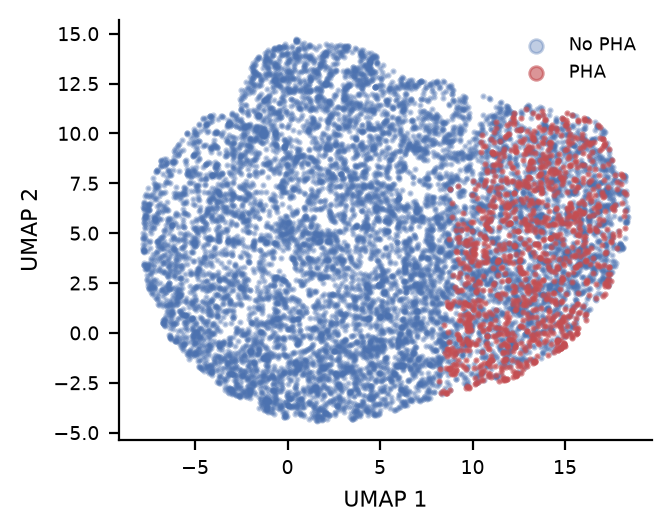
\includegraphics[width=0.85\columnwidth]{figuras/fig5_umap.png}
\caption{Proyección UMAP bidimensional de 12\,000 filas del conjunto de desarrollo, coloreadas por clase.}
\label{fig:umap}
\end{figure}

Con estos resultados se fijó la representación de entrada del modelo definido mediante una regla establecida antes de usar la prueba: se toma la de mayor PR-AUC de validación y, si otra con menos dimensiones queda dentro de su intervalo de confianza, se prefiere la más simple. Solo la selección de tres variables cumple esa condición, de modo que el modelo definido usa $H$, velocidad y distancia de paso, con un 40\,\% menos de variables que la base original.

% =====================================================================
\section{Evaluación final en prueba}
\label{sec:prueba}

Con todas las decisiones tomadas sobre el desarrollo, el modelo definido es un Random Forest de 150 árboles con profundidad máxima 5, hoja mínima de 50 filas y 3 variables por división, entrenado con pesos $1/n$ sobre $H$, la velocidad y la distancia de paso; la probabilidad de cada asteroide es el máximo de las de sus aproximaciones, y el umbral de decisión, 0.333, maximiza $F_1$ en validación. Este modelo se reentrenó con todo el conjunto de desarrollo y se evaluó una única vez en los 5\,485 asteroides de prueba, de los cuales 434 son PHA (Tabla~\ref{tab:prueba} y Fig.~\ref{fig:final}).

\begin{table*}[t]
\centering
\caption{Evaluación final en prueba, por asteroide, con IC 95\,\% por \emph{bootstrap} de asteroides. El Random Forest definido es el único modelo evaluado en prueba; las dos referencias se ajustaron con el desarrollo. Exactitud del clasificador trivial (todo no PHA): 0.921.}
\label{tab:prueba}
\footnotesize
\setlength{\tabcolsep}{3pt}
\resizebox{\textwidth}{!}{%
\begin{tabular}{@{}lcccccc@{}}
\toprule
Modelo & PR-AUC & ROC-AUC & $F_1$ & Precisión & Recall & Exactitud\\
\midrule
Random Forest definido & 0.669 [0.632, 0.707] & 0.952 [0.945, 0.958] & 0.591 [0.553, 0.625] & 0.528 [0.489, 0.568] & 0.671 [0.624, 0.711] & 0.927 [0.920, 0.934]\\
\quad Validación del mismo modelo & 0.698$\pm$0.006 & 0.953$\pm$0.003 & 0.605$\pm$0.015 & 0.549$\pm$0.039 & 0.676$\pm$0.025 & 0.930$\pm$0.007\\
Solo $H$ (reg. log.) & 0.240 [0.211, 0.271] & 0.859 [0.848, 0.869] & 0.387 [0.360, 0.409] & 0.240 [0.220, 0.257] & 0.991 [0.980, 0.998] & 0.751 [0.739, 0.763]\\
Constante (todo PHA) & 0.079 [0.072, 0.086] & 0.500 [0.500, 0.500] & 0.147 [0.135, 0.158] & 0.079 [0.072, 0.086] & 1.000 [1.000, 1.000] & 0.079 [0.072, 0.086]\\
\bottomrule
\end{tabular}}
\end{table*}

En prueba el modelo alcanza un ROC-AUC de 0.952, una PR-AUC de 0.669 y un $F_1$ de 0.591, valores que coinciden con los de validación o quedan muy cerca de ellos; la PR-AUC, la más exigente, baja 0.03, dentro de su intervalo. Esa coincidencia es la comprobación de que el procedimiento funcionó: como la prueba no intervino en ninguna decisión, su resultado estima sin sesgo el desempeño en asteroides nuevos. Al umbral elegido, el modelo detecta 291 de los 434 PHA (recall 0.671) y genera 260 falsas alarmas entre 5\,051 asteroides no peligrosos, de modo que algo más de la mitad de sus alarmas son reales; su exactitud, 0.927, supera ligeramente al clasificador trivial, que no detecta ninguno. Frente al modelo que solo usa $H$, la mejora es grande en todas las métricas que no dependen del umbral (PR-AUC 0.669 frente a 0.240). Dentro del grupo $H\le22$, donde está toda la incertidumbre, el modelo conserva un ROC-AUC de 0.83, mientras que $H$ sola no tiene señal (0.48). Las mismas predicciones, leídas por aproximación en lugar de por asteroide, dan un ROC-AUC de 0.906 y una PR-AUC de 0.468, similares a los mejores modelos por fila: la ganancia del modelo definido está en tratar al asteroide como unidad.

\begin{figure*}[t]
\centering
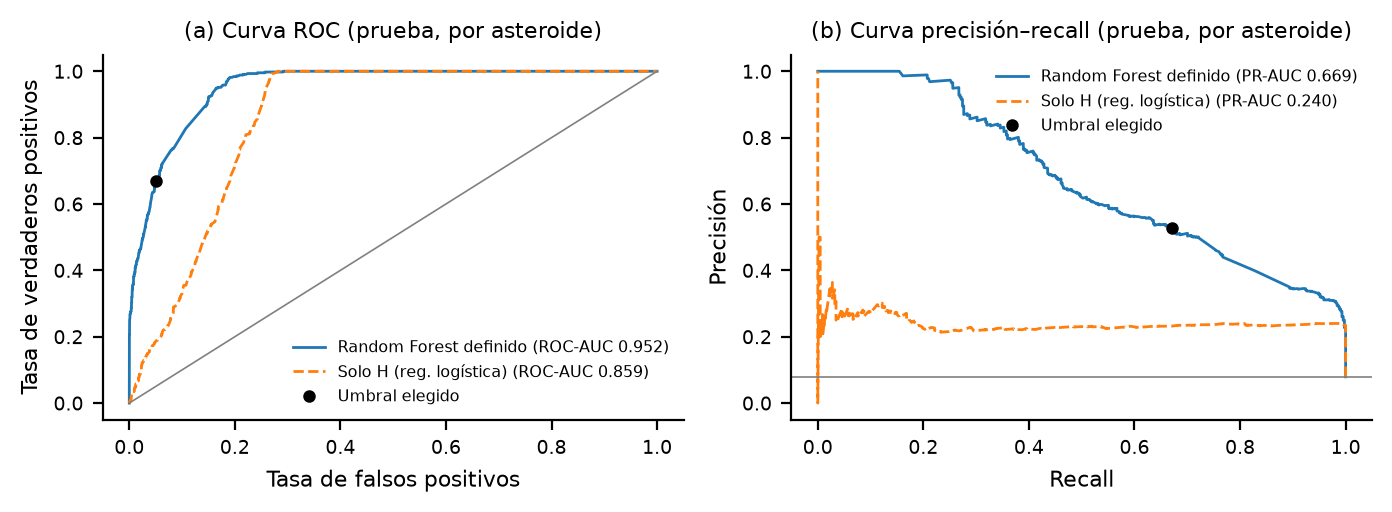
\includegraphics[width=0.85\textwidth]{figuras/fig_final.png}
\caption{Curvas ROC y precisión--recall del Random Forest definido en la prueba, por asteroide, junto a la referencia que solo usa $H$. El punto negro marca el umbral elegido en validación; la línea gris, el desempeño al azar.}
\label{fig:final}
\end{figure*}

% =====================================================================
\section{Discusión y conclusiones}
\label{sec:conclusiones}

Con las variables disponibles, familias muy distintas de modelos llegan prácticamente al mismo desempeño cuando cada aproximación se trata por separado, lo que sugiere que el límite está en los datos y no en el algoritmo. Lo que cambia el resultado es reconocer la estructura de la base. Cada asteroide aparece varias veces, y esa repetición se trató en tres niveles: al partir los datos, agrupando por \code{id} para evitar la fuga que infla las métricas; al entrenar, ponderando cada asteroide por igual, lo que mejora poco las métricas pero lleva a modelos más simples; y al predecir, agregando las probabilidades de sus aproximaciones, que es la decisión que más aporta. En particular, tomar el máximo en lugar del promedio sube la PR-AUC de validación del Random Forest de 0.61 a 0.70, porque una sola aproximación cercana es la evidencia más fuerte de que el MOID es pequeño.

El modelo definido, un Random Forest con tres variables ($H$, velocidad y distancia de paso), pesos $1/n$ y agregación por máximo, alcanza en asteroides nunca vistos un ROC-AUC de 0.952, una PR-AUC de 0.669 y un $F_1$ de 0.591, en línea con su validación. En la práctica, si se usara para priorizar el seguimiento, detectaría dos de cada tres PHA y algo más de la mitad de los objetos que señala serían realmente peligrosos. Frente a un clasificador que solo usa $H$, la mejora es grande en PR-AUC (0.669 frente a 0.240). Este resultado se obtuvo con la prueba reservada hasta el final: todas las comparaciones, la ampliación de la malla, la elección de la agregación y la de la representación se hicieron con validación.

El techo de desempeño se explica por la definición misma de PHA. La etiqueta exige $H\le22$ y un MOID de 0.05\,ua o menos, y la base contiene $H$ pero no el MOID; las aproximaciones cercanas permiten certificar alrededor de una cuarta parte de los asteroides PHA, y el resto depende de elementos orbitales ausentes, de modo que superar el techo exigiría añadirlos. En cuanto a la dimensión, las cinco variables contienen solo tres independientes. Seleccionarlas reduce un 40\,\% las variables sin pérdida, mientras que PCA, aunque encuentra la misma dimensión, perjudica al Random Forest al rotar los ejes, y UMAP no mejora en ningún caso. La distancia de paso, que por sí sola parece irrelevante, resulta la variable más importante en combinación con $H$.

El trabajo tiene limitaciones. El SVM se entrenó con una submuestra de 25\,000 filas; los intervalos de validación con cinco pliegues son amplios, de modo que varias diferencias entre modelos no son significativas; la evaluación final usa un único conjunto de prueba; y la ampliación de la malla y la elección de la agregación se hicieron solo para el modelo definido, no para las demás familias.

\begin{thebibliography}{99}
\bibitem{cneos} NASA/JPL Center for Near Earth Object Studies, ``NEO groups,'' \url{https://cneos.jpl.nasa.gov/about/neo_groups.html} (consultado en nov. de 2026).
\bibitem{chelyabinsk} The Planetary Society, ``What was the Chelyabinsk meteor event?,'' \url{https://www.planetary.org/articles/what-was-the-chelyabinsk-meteor-event} (consultado en nov. de 2026).
\bibitem{nasem2019} National Academies of Sciences, Engineering, and Medicine, \emph{Finding Hazardous Asteroids Using Infrared and Visible Wavelength Telescopes}. Washington, DC: The National Academies Press, 2019, doi:10.17226/25476.
\bibitem{nrc2010} National Research Council, \emph{Defending Planet Earth: Near-Earth-Object Surveys and Hazard Mitigation Strategies}. Washington, DC: The National Academies Press, 2010, doi:10.17226/12842.
\bibitem{kaggle} S. Vani, ``NASA -- Nearest Earth Objects,'' Kaggle, 2022. \url{https://www.kaggle.com/datasets/sameepvani/nasa-nearest-earth-objects} (consultado en nov. de 2026).
\bibitem{fo32} NASA Jet Propulsion Laboratory, ``Asteroid 2001 FO32 will safely pass by Earth March 21,'' mar. 2021. \url{https://www.jpl.nasa.gov/news/asteroid-2001-fo32-will-safely-pass-by-earth-march-21/}
\bibitem{da14} NASA Jet Propulsion Laboratory, ``Small asteroid to whiz past Earth safely,'' feb. 2013. \url{https://www.jpl.nasa.gov/news/small-asteroid-to-whiz-past-earth-safely/}
\bibitem{eros} EarthSky, ``Asteroid Eros at its closest since 1975 on January 31,'' ene. 2012. \url{https://earthsky.org/space/asteroid-eros-at-its-closest-since-1975-on-january-31/}
\bibitem{malakouti} S. M. Malakouti, M. B. Menhaj, and A. A. Suratgar, ``Machine learning techniques for classifying dangerous asteroids,'' \emph{MethodsX}, vol. 11, Art. no. 102337, 2023, doi:10.1016/j.mex.2023.102337.
\bibitem{wang} Y. Wang, ``Comparison of machine learning strategies in hazardous asteroids prediction,'' \emph{Highlights Sci. Eng. Technol.}, vol. 39, pp. 201--208, 2023, doi:10.54097/hset.v39i.6527.
\bibitem{buana} A. Buana, J. Lee, T. D. Quy, and R. Asyrofi, ``Hazardous asteroids classification,'' arXiv:2409.02150, 2024.
\bibitem{baimam} B. B. J. Baimam, ``Explainable deep-learning based potentially hazardous asteroids classification using graph neural networks,'' arXiv:2504.18605, 2025.
\bibitem{sklearn} F. Pedregosa \emph{et al.}, ``Scikit-learn: Machine learning in Python,'' \emph{J. Mach. Learn. Res.}, vol. 12, pp. 2825--2830, 2011.
\bibitem{umap} L. McInnes, J. Healy, N. Saul, and L. Großberger, ``UMAP: Uniform manifold approximation and projection,'' \emph{J. Open Source Softw.}, vol. 3, no. 29, p. 861, 2018, doi:10.21105/joss.00861.
\end{thebibliography}

\end{document}
